%%%%%%%%%%%%%%%%%%%%%%%%%%%%%%%%%%%%%%%%%
% Short Sectioned Assignment
% LaTeX Template
% Version 1.0 (5/5/12)
%
% This template has been downloaded from:
% http://www.LaTeXTemplates.com
%
% Original author:
% Frits Wenneker (http://www.howtotex.com)
%
% License:
% CC BY-NC-SA 3.0 (http://creativecommons.org/licenses/by-nc-sa/3.0/)
%
%%%%%%%%%%%%%%%%%%%%%%%%%%%%%%%%%%%%%%%%%

%----------------------------------------------------------------------------------------
% PACKAGES AND OTHER DOCUMENT CONFIGURATIONS
%----------------------------------------------------------------------------------------

\documentclass[11pt]{article} % A4 paper and 11pt font size

\usepackage[a4paper,margin=1in,footskip=.3in]{geometry}

\linespread{1.0} % Line spacing

\setlength\parindent{0pt} % Removes all indentation from paragraphs - comment this line for an assignment with lots of text
\setlength{\parskip}{6pt}

\usepackage{sectsty} % Allows customizing section commands
\allsectionsfont{\centering \normalfont\scshape} % Make all sections centered, the default font and small caps

\usepackage{fancyhdr} % Custom headers and footers
\pagestyle{fancyplain} % Makes all pages in the document conform to the custom headers and footers
\fancyhead{} % No page header - if you want one, create it in the same way as the footers below
\fancyfoot[L]{} % Empty left footer
\fancyfoot[C]{} % Empty center footer
\fancyfoot[R]{\thepage} % Page numbering for right footer
\renewcommand{\headrulewidth}{0pt} % Remove header underlines
\renewcommand{\footrulewidth}{0pt} % Remove footer underlines
\setlength{\headheight}{13.6pt} % Customize the height of the header

\usepackage[utf8]{inputenc}
\usepackage[T1]{fontenc} % Use 8-bit encoding that has 256 glyphs

\usepackage{fourier} % Use the Adobe Utopia font for the document - comment this line to return to the LaTeX default
\usepackage[english]{babel} % English language/hyphenation

\usepackage{amsmath,amsfonts,amsthm} % Math packages
\theoremstyle{plain}
\newtheorem{theorem}{Theorem}[section]
\newtheorem{corollary}{Corollary}[theorem]
\newtheorem{proposition}[theorem]{Proposition}
\newtheorem{lemma}[theorem]{Lemma}

\theoremstyle{definition}
\newtheorem{definition}{Definition}[section]

\theoremstyle{remark}
\newtheorem*{remark}{Remark}

\numberwithin{equation}{section} % Number equations within sections (i.e. 1.1, 1.2, 2.1, 2.2 instead of 1, 2, 3, 4)
\numberwithin{figure}{section} % Number figures within sections (i.e. 1.1, 1.2, 2.1, 2.2 instead of 1, 2, 3, 4)
\numberwithin{table}{section} % Number tables within sections (i.e. 1.1, 1.2, 2.1, 2.2 instead of 1, 2, 3, 4)

\usepackage{algpseudocode}
\usepackage{algorithm}

\usepackage{listings}

\usepackage{tikz}

\usepackage{natbib}
\bibliographystyle{plainnat}

\usepackage{lipsum} % Used for inserting dummy 'Lorem ipsum' text into the template

\usepackage{siunitx}

\usepackage{float}
\usepackage{wrapfig}
\usepackage{graphicx}

\usepackage{multirow}
\usepackage{booktabs}
\usepackage{array}

\usepackage{url}

\usepackage{hyperref}
\hypersetup{
    colorlinks,
    citecolor=black,
    filecolor=black,
    linkcolor=black,
    urlcolor=black
}
\usepackage{cleveref}
\usepackage{microtype}

\usepackage{todonotes}

% \usepackage{titling}
% \setlength{\droptitle}{-5em}

%----------------------------------------------------------------------------------------
% TITLE SECTION
%----------------------------------------------------------------------------------------

\newcommand{\horrule}[1]{\rule{\linewidth}{#1}} % Create horizontal rule command with 1 argument of height

\title{ 
\normalfont \normalsize 
% \textsc{university, school or department name} \\ [25pt] % Your university, school and/or department name(s)
\horrule{0.5pt} \\[0.4cm] % Thin top horizontal rule
\Large Computer Vision Project (Part 2) \\ [0.1cm] % The assignment title
\large COMP9517 - Semester 1, 2015 \\ [0.2cm]
\horrule{2pt} \\[0.5cm] % Thick bottom horizontal rule
}

\author{
  Louis Tiao \\
  (\texttt{3390558})
  \and
  Edward Lee\\
  (\texttt{3376371})
} % Your name

\date{\normalsize\today} % Today's date or a custom date

\begin{document}

\maketitle % Print the title

\section{Overview}

Facial recognition is an example of a task which is relatively easy for humans but a much more difficult tasks for computers. In this assignment, we compare several different methods for facial recognition as well as assessing their suitability in several specific facial recognition tasks.

\section{Problem Statement}

\todo{I jumped the gun and selected a few small subtasks. Feel free to change these as needed.}

\textbf{Facial Recognition System:} The first part of this project involves designing multiple systems to best match a given image with those in a large database. The facial recognition techniques used include:
  \begin{itemize}
    \item feature-based matching \citep{krivzaj2010adaptation}
    \item template-based matching
    \item appearance-based matching
    \item eigenfaces \citep{turk1991eigenfaces}
  \end{itemize}
We will also benchmark each system to enable us to compare performance in recognizing a series of test images. We supplement our analysis by attempting to implement the following extensions using the technique we deem most suitable.

\begin{enumerate}
    \item \textbf{Facial Verification/Facial Search Engine:} The first extension is to generate a ranking system which assigns a score of similarity between a given facial image and all images in a database. The Facial Search Engine simply extends this ranking system to video inputs.
  % \item \textbf{Facial Verification/Facial Search Engine:} Using the previous recognition system as a starting points, design and implement a program which is able to assign a confidence score of similarity between a given face and faces in the known database. The Facial Search Engine would be the same scoring output, but with an input of a video. The program would be responsible for detecting if there is a face in the image, and to which face in the database that image is most similar to.
  
  \todo{check details of facial similarity and clustering. Can be changed to the supervised learning classification task}
  
  \item \textbf{Facial Similarity and Clustering:} The clustering of faces based on similarity framed as an unsupervised learning problem. This means that given a large database of unseen images, we will design and implement a program which is able to cluster together faces which share some degree of similarity.
\end{enumerate}

% \todo{Need to nail down a subset the below problems.}

% \begin{itemize}
%   \item Detecting the fact or state of one or more faces appearing in a digital image
%   \item Face verification - confidence score of similarity between faces (biometric security)
%   \item Facial search engine - searching a database of images or videos against a query face.
%   \item Head pose estimation
%   \item Unsupervised learning - Clustering faces given a number of faces
%   \item Supervised learning - classification problems depending on availability of labeled images
%     \begin{itemize}
%       \item Age, Gender
%       \item Mood
%       \item Attractiveness (could build a service that leverages Tinder API, where our software
%       creates a database of attractive and unattractive faces based on right and left swipes respective
%       by computing eigenfaces, and then automates swipes once enough examples have been seen)
%     \end{itemize}
% \end{itemize}

\section{Literature Survey \& Approach}

\todo{I do think separate Literature Survey and Approach/Method sections may be necessary.}

% Cited works \citep{litvin2003,battiato2007sift,grundmann2011auto,liu2009content,Matsushita2006}

% Section 14.2 Szeliski

% http://www.face-rec.org/

\begin{enumerate}
  \item \textbf{Facial Recognition System:} We wish to implement more than one facial recognition system in order to do comparisons and evaluations on state of the art facial recognition techniques. One common method real-time method from involves the use of Eigenfaces, a low-dimensional representation of facial images, for facial recognition \citep{turk1991eigenfaces}. A more novel method described in \citep{krivzaj2010adaptation} details the use of SIFT feature detection in facial detection. In Part 1 of our project we already used SIFT feature detection on images meaning that we can adapt previous work and compare it to more advanced techniques such as eigenfaces for facial recognition. We will be using the extended yale face database B to begin our investigation, acquiring more datasets as needed. 

  \item \textbf{Facial Verification/Facial Search Engine:} 
  Upon completion of a facial recognition system, we can then adapt it to display 

  \item \textbf{Facial Similarity and Clustering:}
\end{enumerate}

% \section{Approach}

% \begin{enumerate}
%   \item \textbf{Facial Recognition System:} The approach to this part of the assignment will be to compare different implementations for facial recognition. These techniques include feature-based matching, template-based matching and Eigenfaces.
%   \item \textbf{Facial Verification/Facial Search Engine:} 
%   \item \textbf{Facial Similarity and Clustering:}
% \end{enumerate}


% % outline subtasks/problems here

% \begin{itemize}
%   \item feature-based
%   \item template-based
%   \item appearance-based
% \end{itemize}

% Eigenfaces (Section 14.2.1 Szeliski)

% mention which datasets to use, etc.

% Page 719 Szeliski

\section{Plan}

% general plan here

\begin{figure}[ht!]
\centering
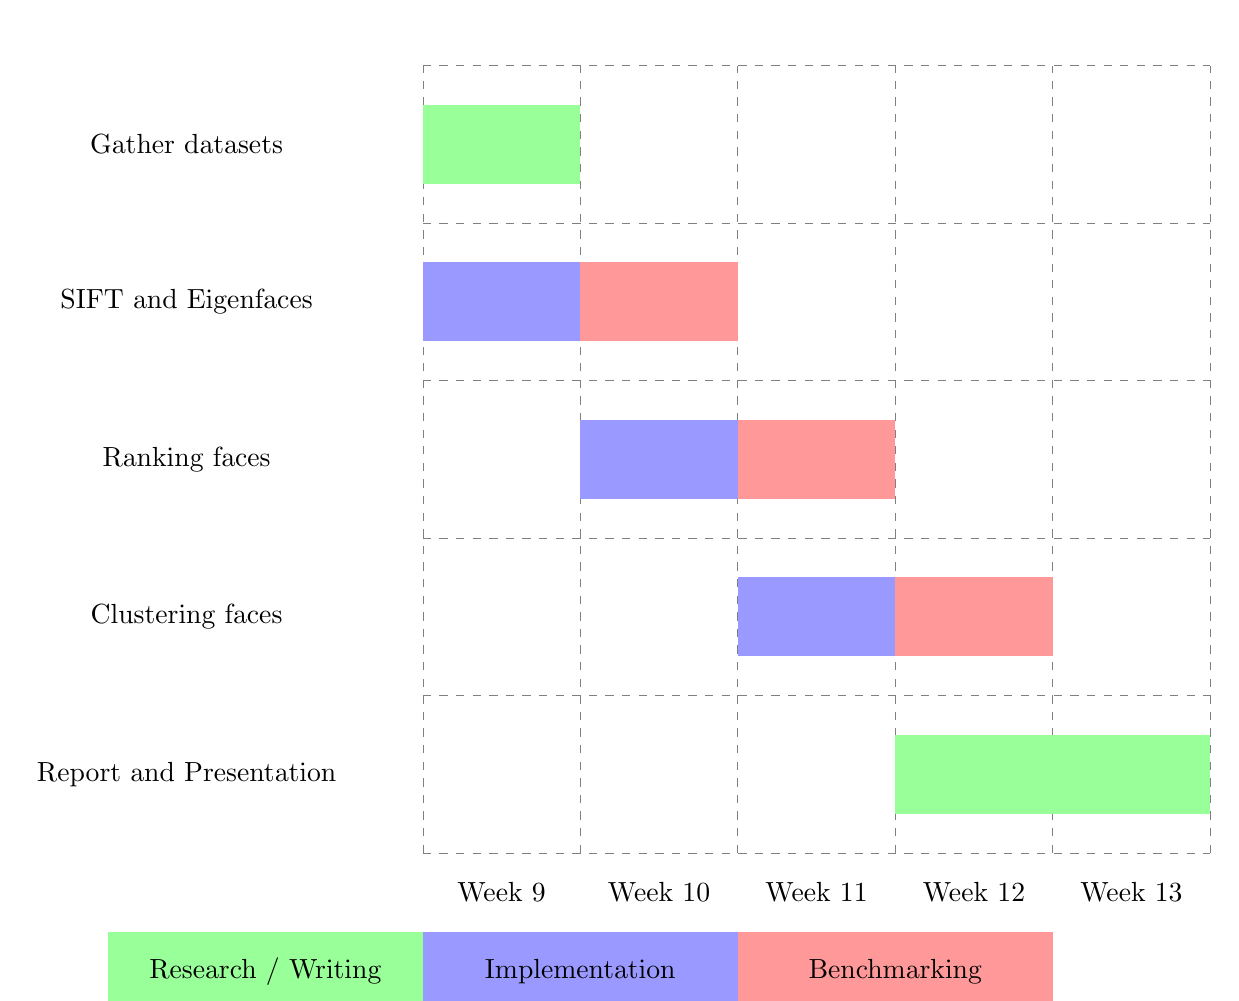
\begin{tikzpicture}[every node/.style={font=\normalsize,
  minimum height=0.5cm,minimum width=0.5cm},]

  \draw[step=2cm,gray,very thin,dashed] (0,0) grid (10,10);
  \node[] at (1,-0.5) {Week 9};
  \node[] at (3,-0.5) {Week 10};
  \node[] at (5,-0.5) {Week 11};
  \node[] at (7,-0.5) {Week 12};
  \node[] at (9,-0.5) {Week 13};

  % datasets
  \node[] at (-3, 9) {Gather datasets};
  \fill[green!40!white] (0,8.5) rectangle (2,9.5);

  % SIFT feature detection + Eigen faces  
  \node[] at (-3, 7) {SIFT and Eigenfaces};
  \fill[blue!40!white] (0,6.5) rectangle (2,7.5);
  \fill[red!40!white] (2,6.5) rectangle (4,7.5);

  % ranking
  \node[] at (-3, 5) {Ranking faces};
  \fill[blue!40!white] (2,4.5) rectangle (4,5.5);
  \fill[red!40!white] (4,4.5) rectangle (6,5.5);

  % clustering
  \node[] at (-3, 3) {Clustering faces};
  \fill[blue!40!white] (4,2.5) rectangle (6,3.5);
  \fill[red!40!white] (6,2.5) rectangle (8,3.5);

  % documentation
  \node[] at (-3, 1) {Report and Presentation};
  \fill[green!40!white] (6,0.5) rectangle (10,1.5);

  % legend
  \fill[green!40!white] (-4, -2) rectangle (0, -1);
  \node[] at (-2, -1.5) {Research / Writing};
  \fill[blue!40!white] (0, -2) rectangle (4, -1);
  \node[] at (2, -1.5) {Implementation};
  \fill[red!40!white] (4, -2) rectangle (8, -1);
  \node[] at (6, -1.5) {Benchmarking};

\end{tikzpicture}
\end{figure}

\bibliography{../bibliography}

%----------------------------------------------------------------------------------------

\end{document}